\section{Implementation}
\label{sec:implementation}

Web application development framework \textit{Django}~\cite{django}, Web API toolkit \textit{Django REST Framework} (DRF)~\cite{drf} and Python~\cite{python} library \textit{django-filter}~\cite{django-filter} are used to operate \boatvtwo.
PostgreSQL~\cite{psql} is used to provide a database for the server-side applications of the software.
During the implementation phase, decisions regarding models of the database have been directed towards the UI utilizing the API for database queries and searches.
The models reflect the \ud\ format of sentences and annotations are saved as fields of word lines.

All the pages of the tool have been supported by Bootstrap~\cite{bootstrap}.
The annotation page has most of the functionalities of \boatvone.
Entries are validated and errors are displayed on the annotation page for annotators to see invalid edits in real time, according to the \ud\ framework~\cite{UD} and the language provided.

Python library \textit{spa\textsc{C}y}~\cite{spacy} is used to provide linear dependency graphs.
Another JavaScript-based linear dependency graph~\cite{spyssalo} making use of \textit{brat}~\cite{brat} is used to provide graphs as well.
An annotator's preference regarding this may vary, thus, giving them visualization options is important.



%\section{Annoations with \boatvtwo}
%\label{sec:features}

As stated in Section~\ref{sec:introduction} \boatvtwo\ aims to support the annotator experience by facilitating faster and correct annotations in a collaborative manner. The following features have been impemented towards this end:

\begin{figure}[tbh]
    \centering
    \tcbox[left=0mm,right=0mm,top=0mm,bottom=0mm,boxsep=1pt,arc=0mm,boxrule=0.5pt,colframe=black,sharp corners]
    {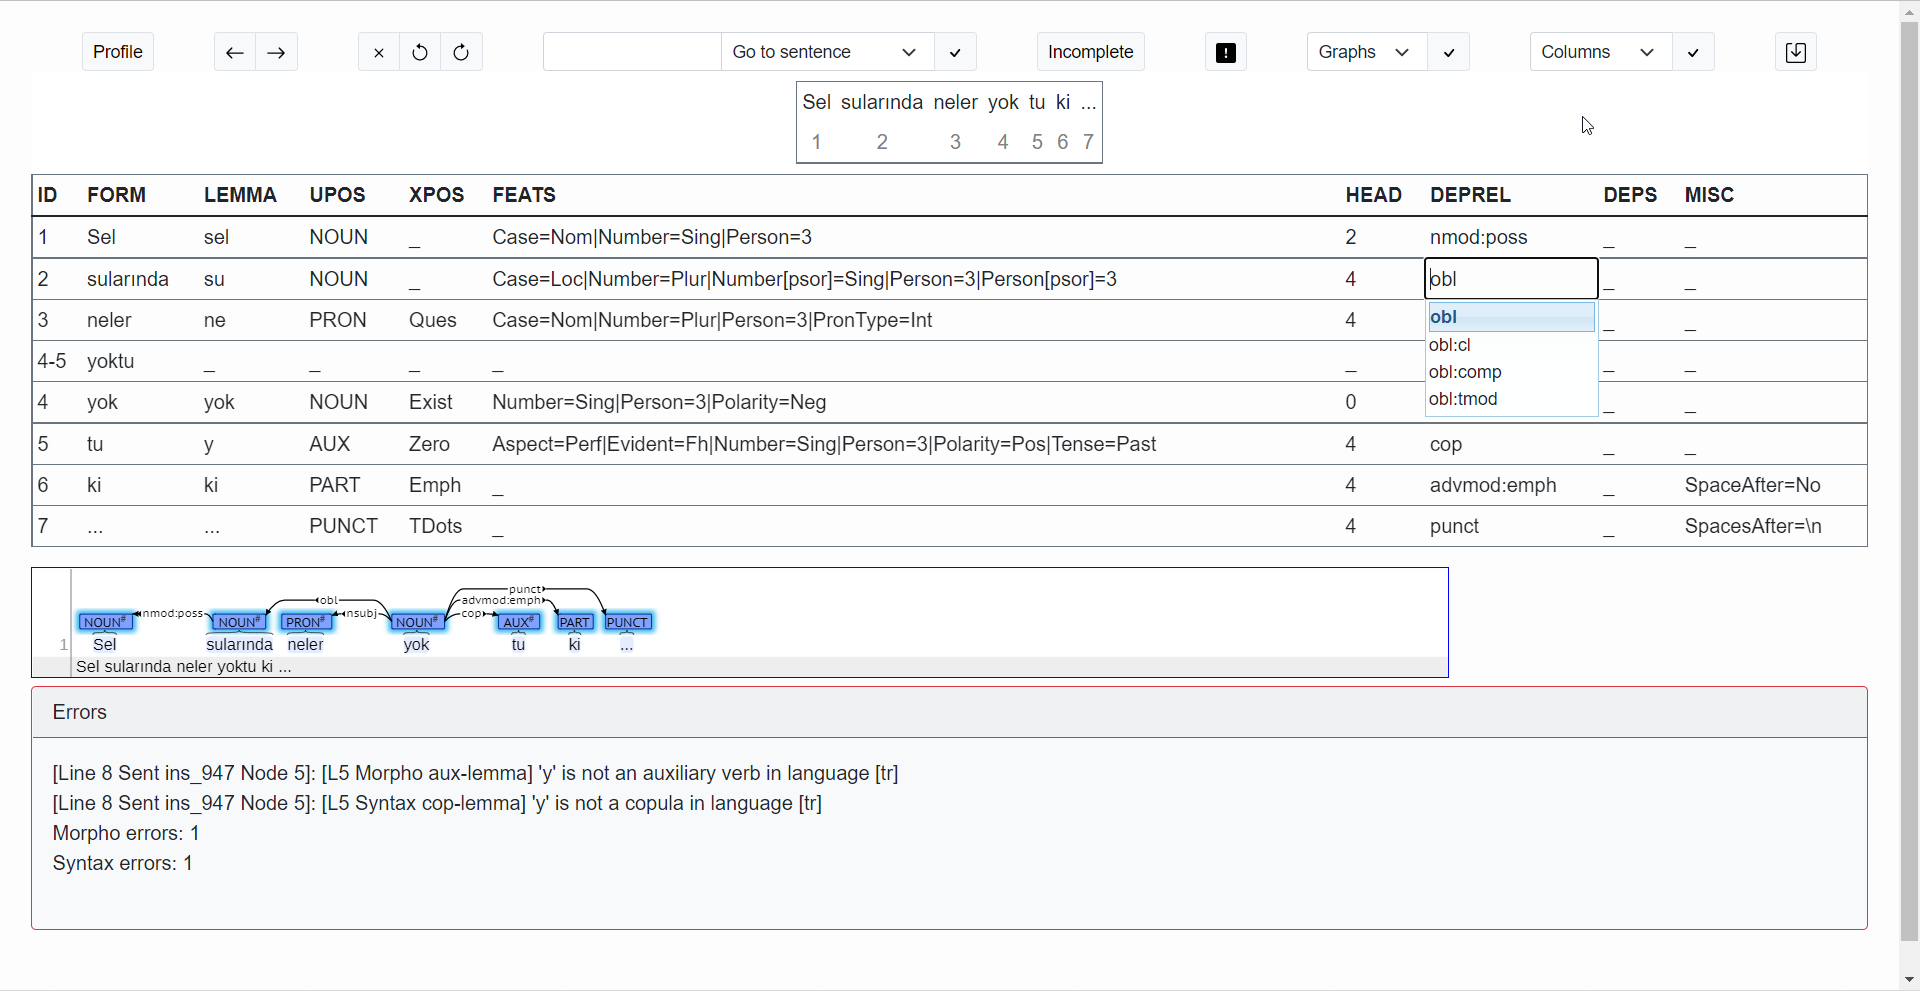
\includegraphics[width=1\textwidth]{figures/sample-annotation.png}}
    \caption{The annotation screen captured while the sentence ``Sel sularında neler yoktu ki...'' is being annotated. The \deprel\ tag for the \form\ ``sularında'' is being annotated by selecting among the valid alternatives that appear in the pop-up. Selections can be made with use of arrow keys.}
    \label{fig:anno-fig}
\end{figure}

\begin{itemize}[before=\normalfont, font=\itshape, align=left]
    \item[Treebanks:]
        Ability to work with multiple treebanks. Users can select which treebank they work on and upload new treebanks as \conllu\ files.  
        Treebanks and their annotations are stored in a database. 

    \item[Annotation view:]
    	The sentence annotation page is very similar to  \boatvone.
    	It consists of three main parts: (1) A table with rows for every lemma in the sentence and columns correpsonding to their annotations  \todo{Explain the tags UPOS, DEPRL etc. }; (2) the dependency graph of the sentence; and (3) UD validation errors. 
    	The dependency graph and errors are syncronized during annotation process. 
        Several  dependency graph presentations are supported to suit the annotator preference. 
        As horizontal graphs can consume a significant amount of screen real-estate, which can lead to loss of focus in long sentences that are common in agglutinative languages. 
        
        As some sentence annotations can be very complicated or an annotator may need to stop the annotation process for some reason, there is a need for capturing the state of the annotation for a given sentence by a given annotator. For this purpose, each sentence is assigned a status that may be:    ``incomplete", ``draft" and ``complete". A user can continue with an incomplete 
       The status of an annotation is also shown in the search view to assist the user. 
       
       The annotator is able to perform almost all operations via keyboard action.
       This was a strong request from annotators, which they were very please with and reported improved flow and greatly improved speed.
       The desire for operating from the keyboard arises from the need to annotate a great many features for agglutinative languages, where most lemmas get annotated. Drag and drop interfaces force annotatators to toggle back and forth between mouse and keyboard interactions which were reported to be very frustrating in terms of concentration and speed. 
       
       Figure~\ref{fig:anno-fig} shows the annotation view while an annotator is annotating a Turkish sentence ( ``Sel sularında neler yoktu ki...''). 
        
    \item[Improved searching for reference and consistency:]
    	Due to the complexity of some kinds of annotations it is very useful for an annotator to be able to refer to previously made annotations.
    	Such annotations may be made by the same or other annotator. 
    	As this applicaiton supports multiple users, annotators are able to share experiences.

        The utility of this feature can be described with a real case during the annotation of a sentence related to a Zodiac sign (noun). \todo{Put the real Turkish example here}
        Being unsure about how to annotate its \upos\ tag, she manually searched the \conllu\ file for similar cases and discovered that it had been  annotated in two different manners previously (inconsistency).  

        Another example of difficult references involve the  \textit{-ki} morpheme in Turkish.
        For example, in the sentence ``Evdeki halılar yıkandı.'' (\textit{The rugs at home were washed.}), the \textit{-ki} acts as an adjectivizer.
        However, in ``Benim halılarım yün, Ayşeninkiler sentetik.'' (\textit{My rugs are woolen. Ayşe's are synthetic.}), it is pronominal.
        Searching for sentences where the  \textit{-ki} morpheme occurs for a reference would be hopeless with text search as they occur very frequently.
        In MRLs this is a common occurrance. 
        
        Since manual search is difficult in \conllu\ files, even if regular expressions are used due to ambiguities, we have implemented text, regular expression, and \ud\ tag based searching.   
        This functionality intends to support the creation of more accurate and consistently annotated treebank. 

    \item[Inter-annotator agreement:]
        The inter-annotator agreement is needed to check the consistency of annotations among annotators. 
		Since this tool keeps track of annotations made by annotators, such computations are easily supported. 



\end{itemize}
